\chapter{The Protocol} % Main chapter title

\label{Chapter4} % Change X to a consecutive number; for referencing this chapter elsewhere, use \ref{ChapterX}


\section{Introduction}

Designing a sound-based protocol for tracking the moves of a Rubik's
Cube requires great care. Lots of things produce sound that could
interfere with the protocol: people talking, machines operating, nature
stirring, and so forth. Furthermore, the structure of the Rubik's Cube
itself imposes stringent physical constraints on the size of any
components used to produce the sounds used in the protocol.

This chapter first seeks to clearly detail the specific constraints
that must be considered when designing a sound-based protocol for
tracking the moves of a Rubik's Cube in Section
\ref{sec:protocol-requirements}. From there, a specific protocol that
meets these constraints will be proposed in Section
\ref{sec:specification}. This proposed protocol will then be contrasted
with an alternative option in Section \ref{sec:alternatives}. Finally,
an overview of the plan to implement the proposed protocol in a
proof-of-concept will be given in Section \ref{sec:protocol-summary}


\section{Requirements}
\label{sec:protocol-requirements}

This section will detail the constraints required for designing a
protocol for tracking the moves of a Rubik's Cube.

These constraints include a sufficiently strong signal-to-noise ratio
(Section \ref{subsec:signal-to-noise-ratio}), sufficient distinctiveness
between tones (Section \ref{subsec:tone-distinctiveness}), the frequency
response range of consumer hardware
(Section \ref{subsec:frequency-response-range}), and the human auditory range
(Section \ref{subsec:human-auditory-range}).

\subsection{Signal-to-Noise Ratio}
\label{subsec:signal-to-noise-ratio}

Sound is an easily accessible, and therefore noisy, medium of
communication. As a result, any data transmission protocol based on
sound must be resilient to the presence of additional noise unrelated
to the signal being transmitted. For a sound-based protocol to be
effective, its tones must be easily distinguishable from background
noise.

For the purpose of this thesis, "background noise" will be considered
the ambient noise present in a quiet room when a speedcuber is actively
solving a Rubik's Cube. Measurement of the background noise was carried
out by using the Android app Spectroid \cite{googleplay-spectroid} to
create live visualizations of the background noise in a household
bedroom (a typical place for a speedcuber to practice solving the cube)
while solving three types of speedcubes selected based on their
"noisiness". A fourth visualization of just the ambient noise in the
bedroom (i.e. while no cubes were being solved) was also recorded as a
control. These visualizations are shown in Figure
\ref{fig:signal-to-noise-ratio}.

% How to do a sub-figure: https://tex.stackexchange.com/a/37597
\begin{figure}
    \centering
    \caption{Background Noise of a Quiet Room while Speedsolving}
    \label{fig:signal-to-noise-ratio}
    \begin{subfigure}{\textwidth}
        \centering
        \caption{No Speedsolving (Quiet Room)}
        \label{fig:signal-to-noise-ratio-silent}
        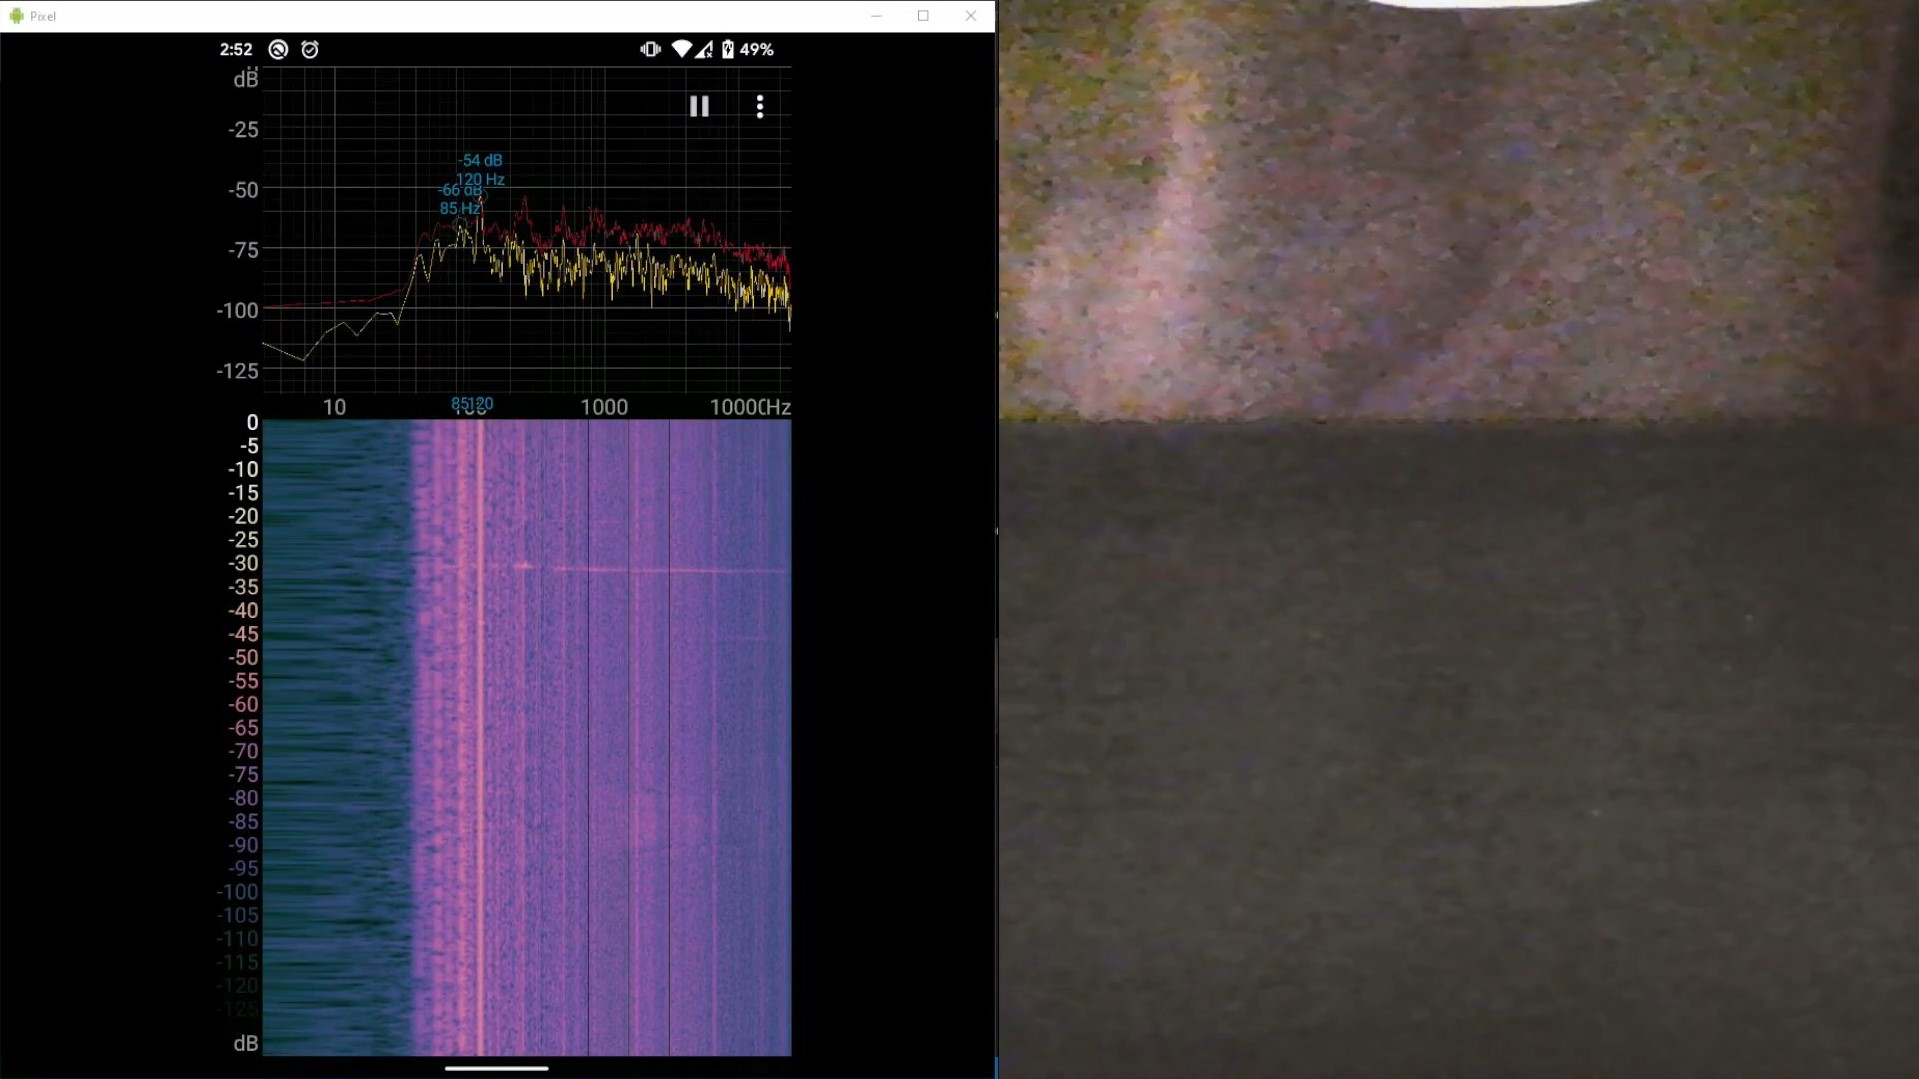
\includegraphics[width=\linewidth]{Figures/4 Protocol Design/Signal to Noise Ratio/silent_background_noise.jpg}
        \vspace*{2mm}
    \end{subfigure}\\
    \begin{subfigure}{\textwidth}
        \centering
        \caption{Quiet Solving (Gans 356)}
        \label{fig:signal-to-noise-ratio-356}
        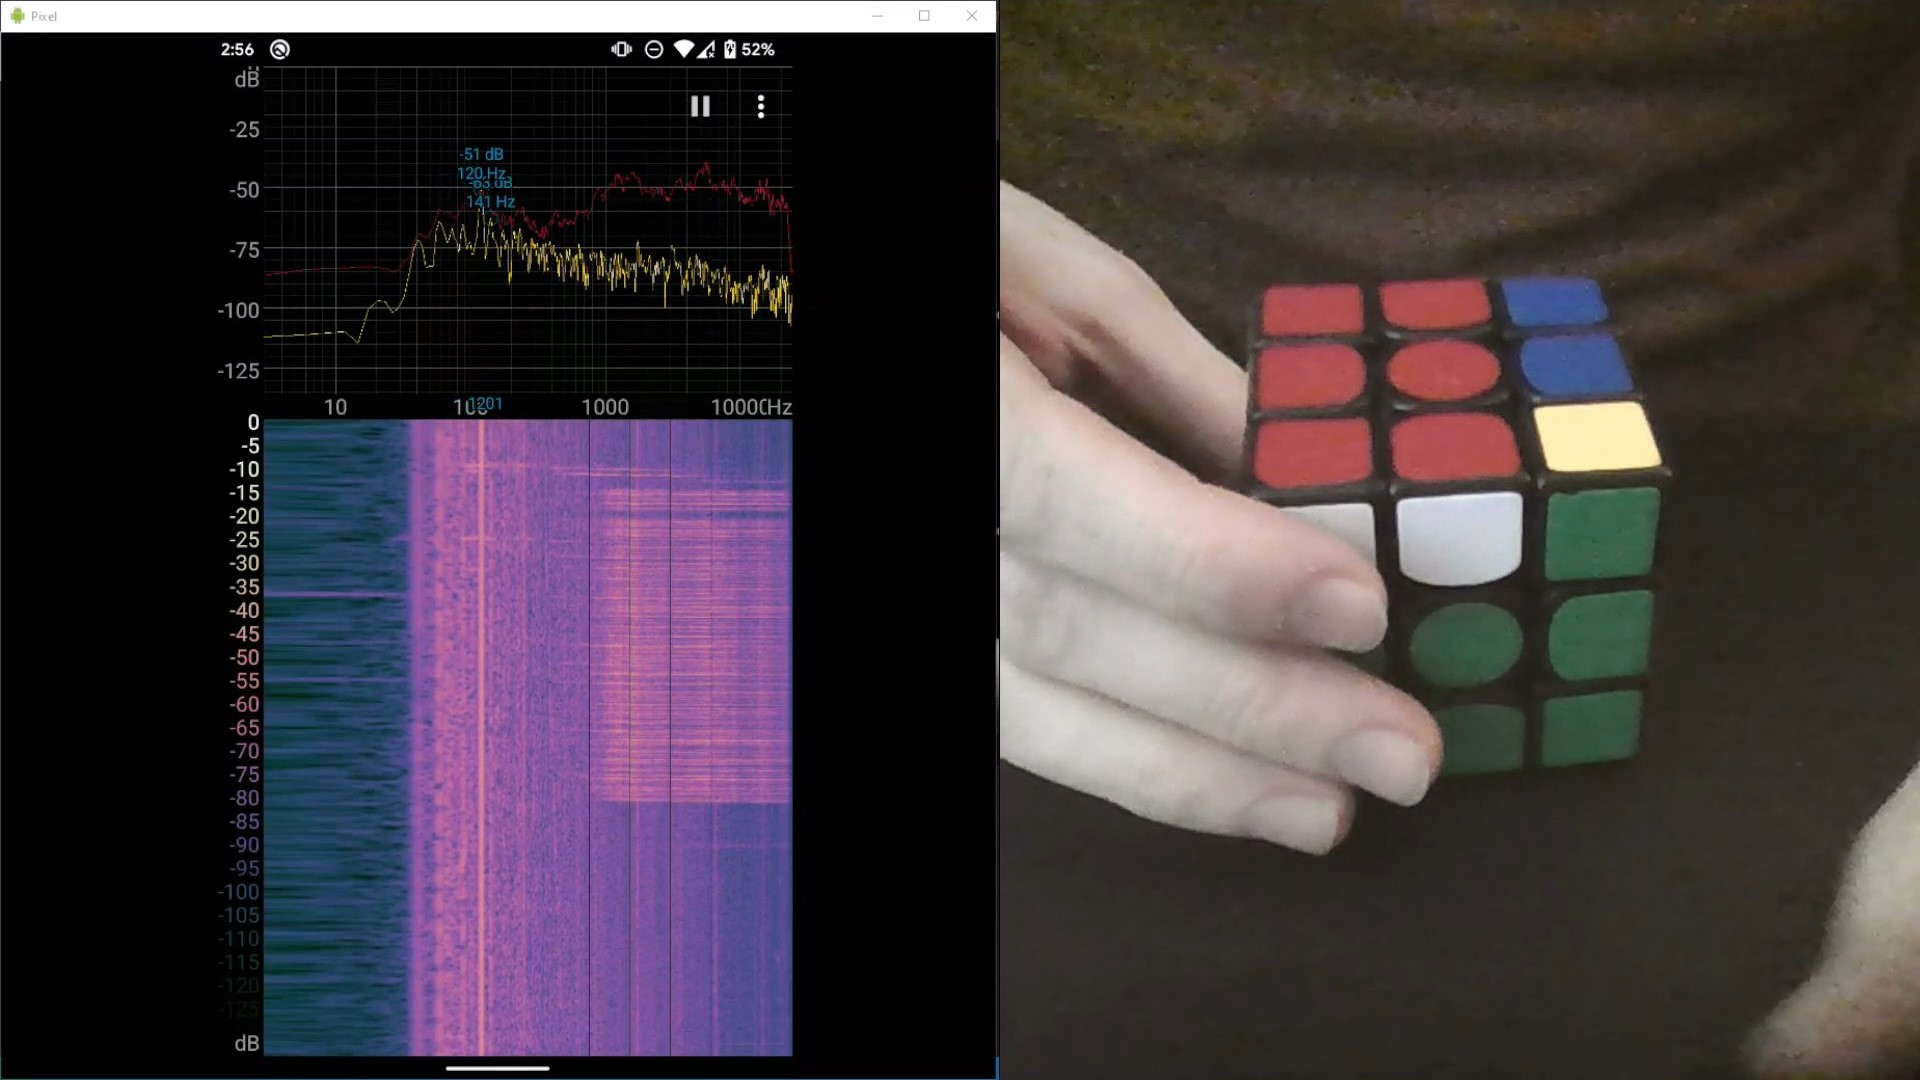
\includegraphics[width=\linewidth]{Figures/4 Protocol Design/Signal to Noise Ratio/356_background_noise.jpg}
        \vspace*{2mm}
    \end{subfigure}
\end{figure}
\begin{figure}\ContinuedFloat
    \centering
    \begin{subfigure}{\textwidth}
        \centering
        \caption{Normal Solving (Gans XS)}
        \label{fig:signal-to-noise-ratio-xs}
        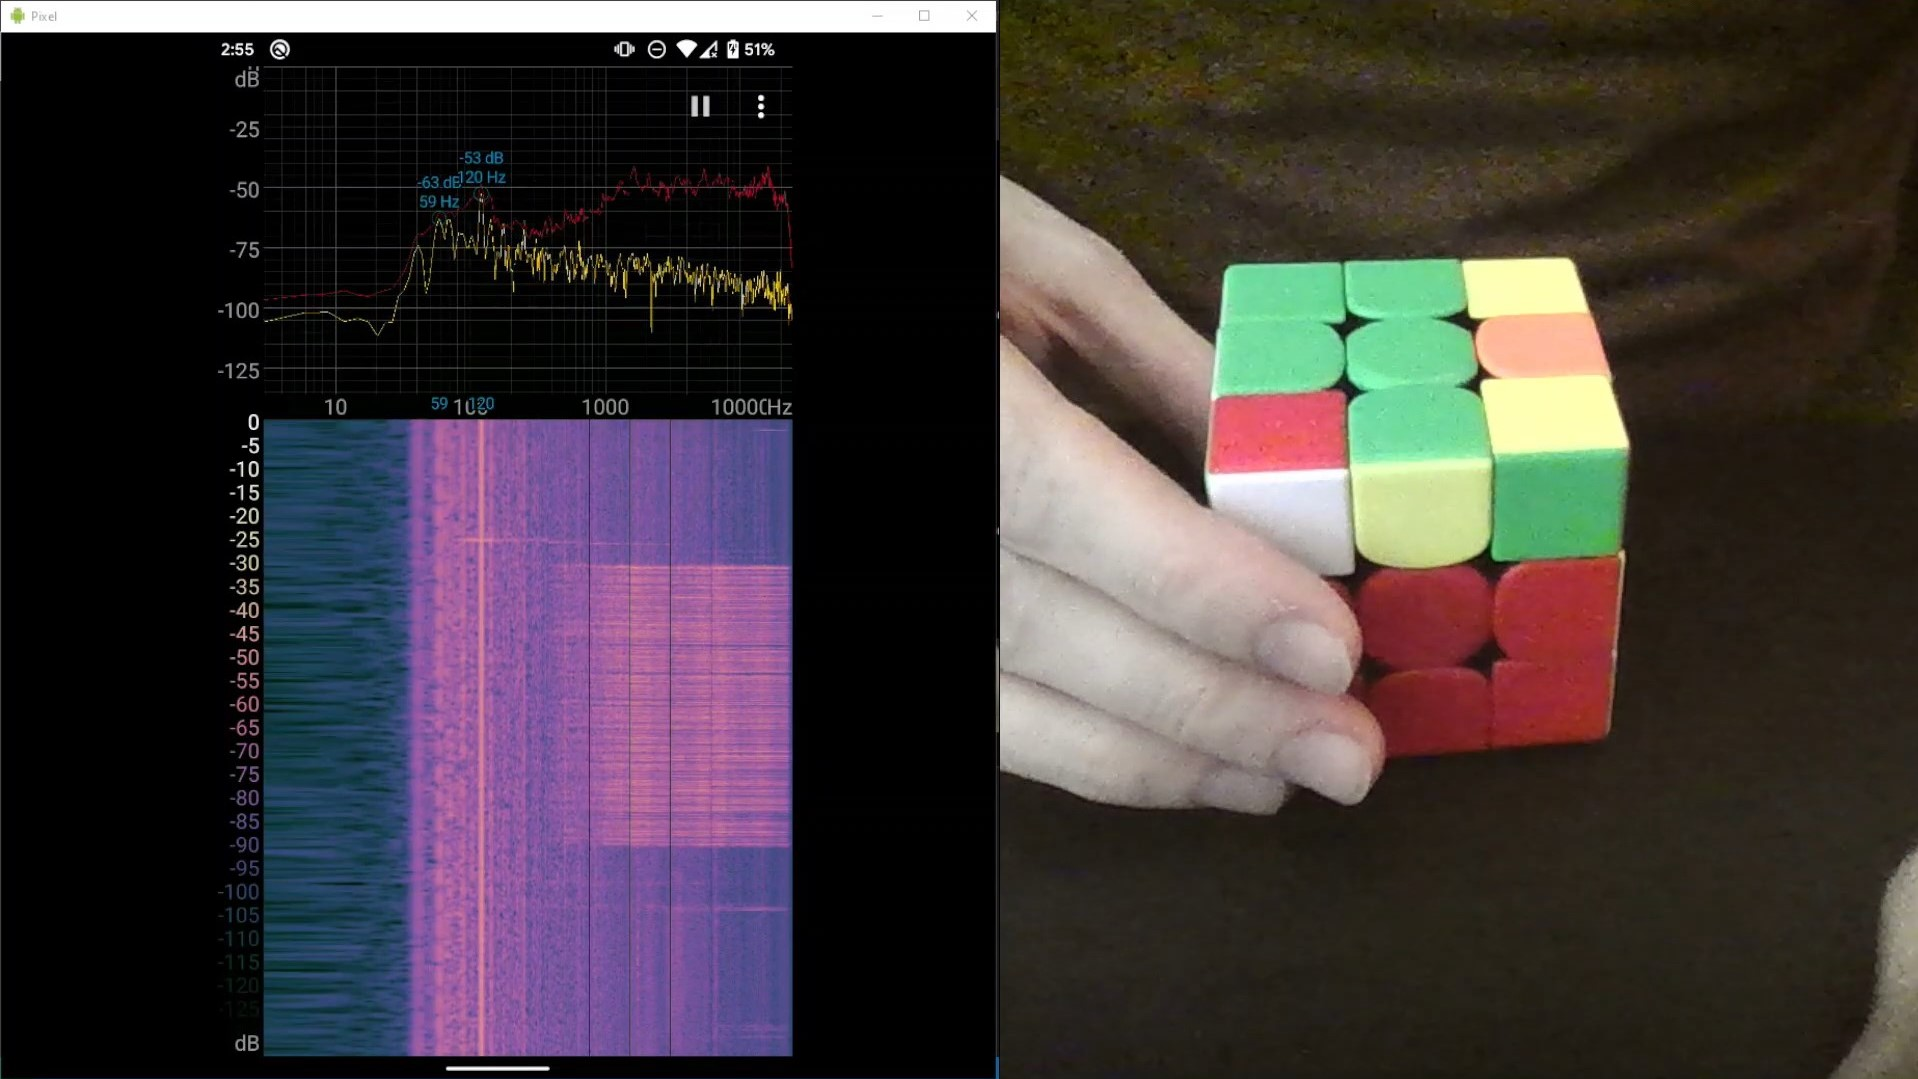
\includegraphics[width=\linewidth]{Figures/4 Protocol Design/Signal to Noise Ratio/xs_background_noise.jpg}
        \vspace*{2mm}
    \end{subfigure}\\
    \begin{subfigure}{\textwidth}
        \centering
        \caption{Loud Solving (QiYi Qimeng)}
        \label{fig:signal-to-noise-ratio-qiyi}
        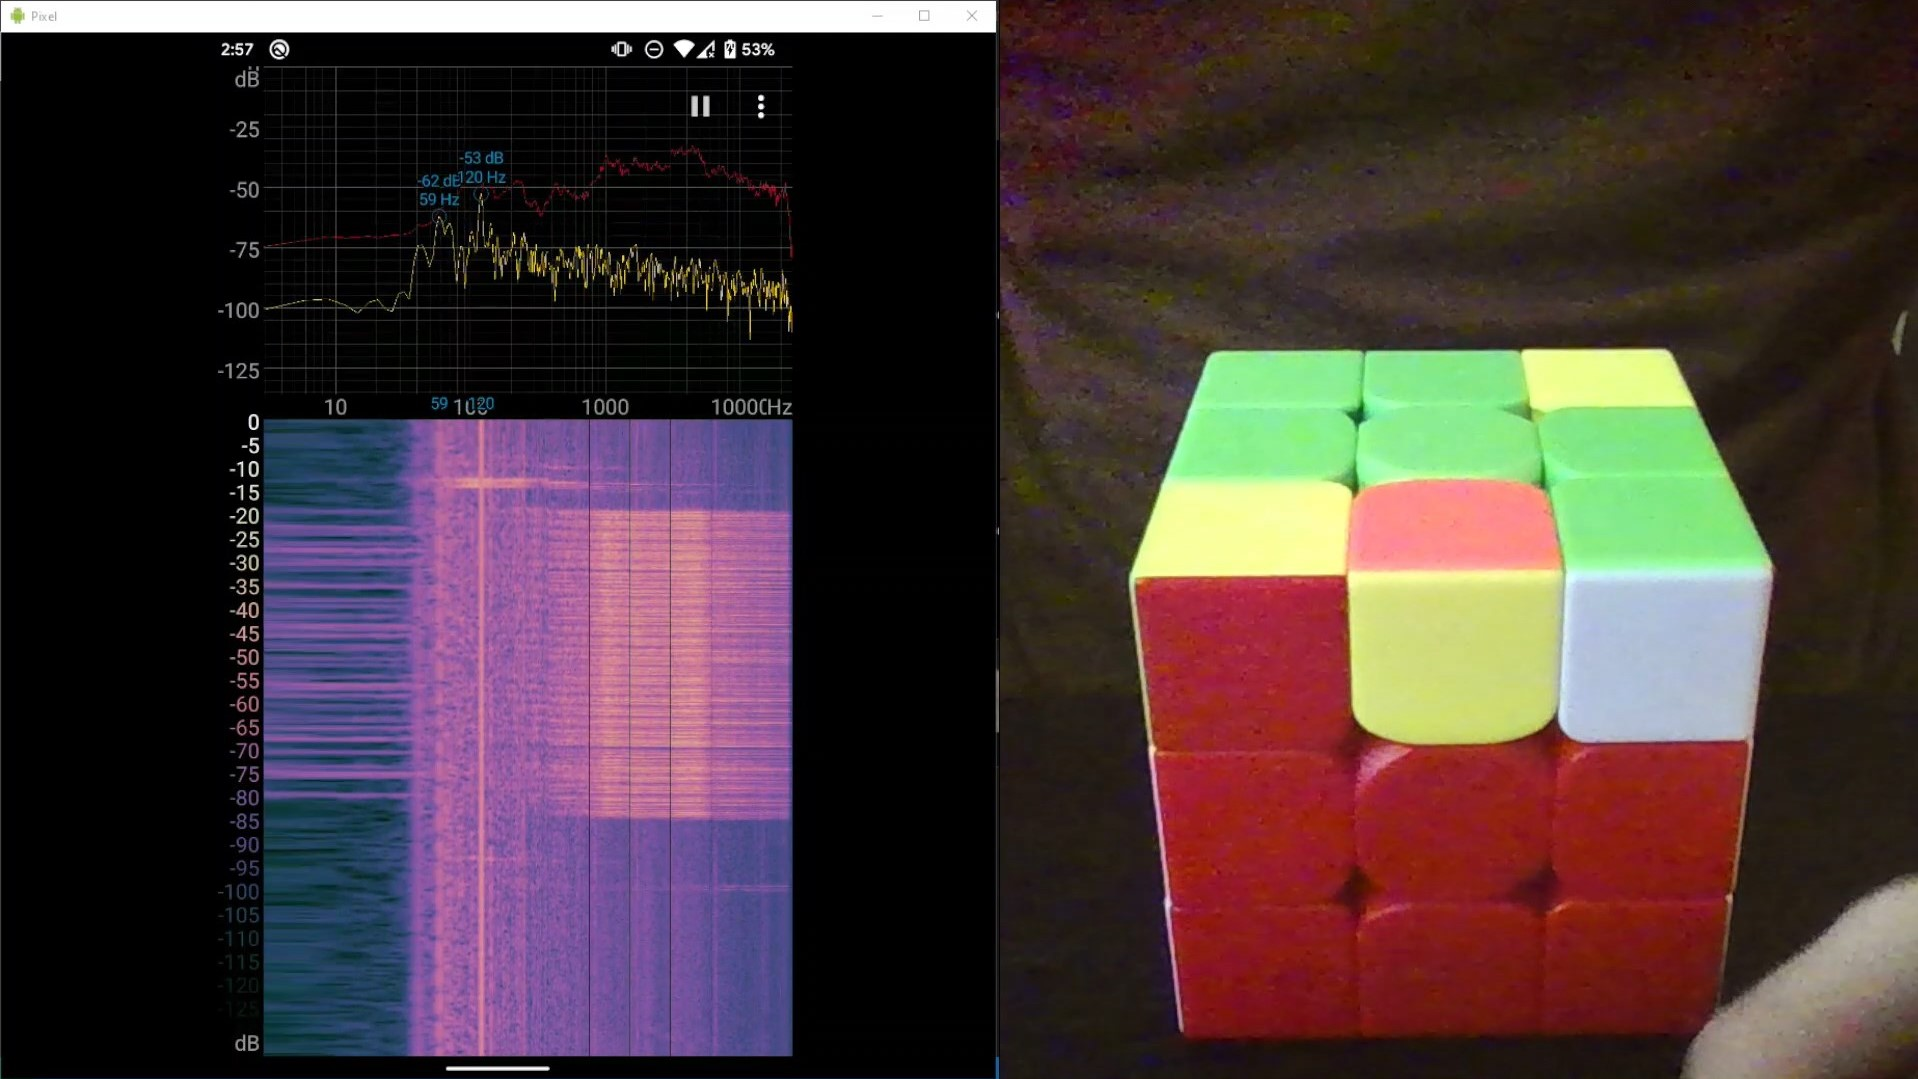
\includegraphics[width=\linewidth]{Figures/4 Protocol Design/Signal to Noise Ratio/qiyi_background_noise.jpg}
        \vspace*{2mm}
    \end{subfigure}%
\end{figure}

\subsubsection{How to Read a Spectrogram}
\label{subsubsec:how-to-read-a-spectrogram}

These visualizations are formally known as an audio "spectrogram", and
show both the specific frequencies present in each audio sample and
their intensity.

The graph on top shows the current and maximum strengths of each
frequency present in the background audio with the yellow and red lines
respectively. The x-axis measures the specific frequencies in Hz, while
the y-axis shows the intensity (aka loudness) of those frequencies in
dB.

The lower graph is the actual spectrogram of the background audio. It
shares the same x-axis as the top graph, but its y-axis instead
measures time with time = 0 at the bottom of the graph and time = now
at the top. Here, the brighter colors represent a more intense (aka
louder) frequency with the exact key shown on the left side of the
graph. As such, this lower graph can be considered a "bird's eye view"
of the top graph over time.

\subsubsection{Key Observations from the Spectrogram}
\label{subsubsec:key-observations-from-the-spectrogram}

As shown in Figure \ref{fig:signal-to-noise-ratio-silent}, the
predominant background noises in a quiet bedroom are the tones between
80Hz - 500Hz which reach a max strength of -54dB.

In contrast, Figures \ref{fig:signal-to-noise-ratio-356} and
\ref{fig:signal-to-noise-ratio-xs} show that solving a speedcube
creates additional noise in the frequency ranges from 1000Hz - 20000Hz,
with Figure \ref{fig:signal-to-noise-ratio-qiyi} showing particular
strength from the noisy QiYi cube with the frequencies in the 1000Hz -
10000Hz range reaching up to -30dB.

Thus, a sound-based move tracking protocol must account for the
following items in order to achieve an adequate signal-to-noise ratio:

\begin{itemize}
    \item Tones between 500Hz and 1000Hz are the easiest to detect while solving a speedcube since they have the least competition from other background sounds while solving a speedcube.
    \item Tones between 1000Hz and 20000Hz must be significantly louder than -30dB or they risk being indistinguishable from the background noise created by a noisy speedcube like the QiYi Qimeng.
\end{itemize}

\subsection{Tone Distinctiveness}
\label{subsec:tone-distinctiveness}

If more than one tone is required for the protocol, each tone must be
unique enough to be easily distinguished from each other tone. Since a
standard smartphone or laptop microphone will be used on the listening
end of this protocol, the definition of "easily distinguishable" must
be based on an assessment of how clearly smartphone and laptop-grade
microphones can distinguish similar frequencies.

To measure the sensitivity of a standard smartphone microphone (in this
case a Google Pixel 1), a recording was taken of two distinct tones
that started 500 Hz apart and stepped closer together in 10 Hz
increments every 0.5 seconds until their frequencies were identical.

As shown in Figure \ref{fig:tone-sep}, the two tones are clearly
distinguishable from 500Hz apart to 150Hz apart. However, the
distinction began waning once the tones came within 100Hz of each
other, and by 80Hz they became entirely indistinguishable.

% How to do a sub-figure: https://tex.stackexchange.com/a/37597
\begin{figure}[h]
    \centering
    \caption{Distinctiveness of Two Increasingly Similar Tones}
    \label{fig:tone-sep}
    \begin{subfigure}{0.5\textwidth}
        \centering
        \caption{500Hz Separation}
        \label{fig:tone-sep-500}
        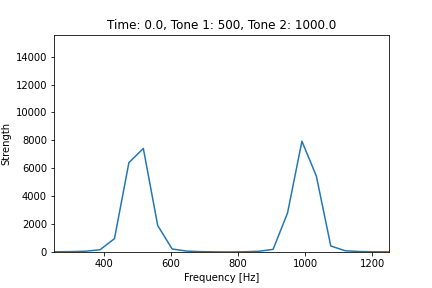
\includegraphics[width=.90\linewidth]{Figures/4 Protocol Design/Tone Distinctiveness/0.06.png}
        \vspace*{2mm}
    \end{subfigure}%
    \begin{subfigure}{0.5\textwidth}
        \centering
        \caption{150Hz Separation}
        \label{fig:tone-sep-150}
        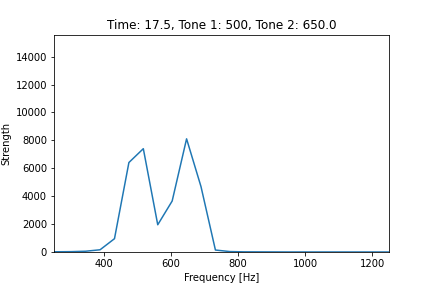
\includegraphics[width=.90\linewidth]{Figures/4 Protocol Design/Tone Distinctiveness/17.53.png}
        \vspace*{2mm}
    \end{subfigure}\\
    \begin{subfigure}{0.5\textwidth}
        \centering
        \caption{100Hz Separation}
        \label{fig:tone-sep-100}
        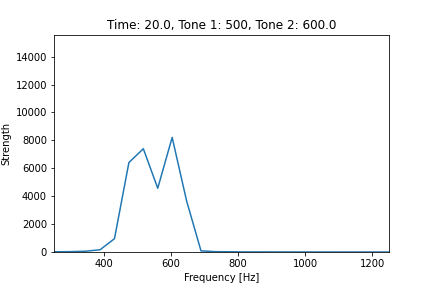
\includegraphics[width=.90\linewidth]{Figures/4 Protocol Design/Tone Distinctiveness/20.03.png}
        \vspace*{2mm}
    \end{subfigure}%
    \begin{subfigure}{0.5\textwidth}
        \centering
        \caption{80Hz Separation}
        \label{fig:tone-sep-80}
        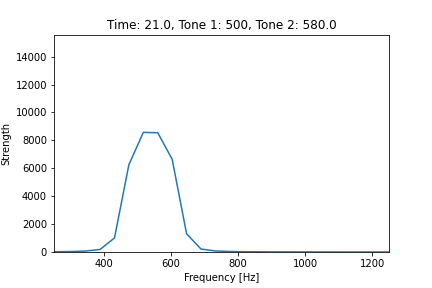
\includegraphics[width=.90\linewidth]{Figures/4 Protocol Design/Tone Distinctiveness/21.01.png}
        \vspace*{2mm}
    \end{subfigure}%
\end{figure}

Thus, a sound-based move tracking protocol must account for the
following items in order to achieve adequate tone distinctiveness:

\begin{itemize}

    \item Tones should be separated by at least 100Hz in order to be
    clearly distinguished from other tones in the protocol.

\end{itemize}


\subsection{Frequency Response Range of Consumer Hardware}
\label{subsec:frequency-response-range}

Since a standard smartphone or laptop microphone will be used on the
listening end of this protocol, any tones used in the protocol must be
within the range of tones that a smartphone or laptop-grade microphones
can pick up, otherwise a more sophisticated, external microphone will
need to be attached to the device. This range is formally known as the
"frequency response range" of the microphone.

According to a Stanford research paper \cite{typical-mic-range} that
analyzed over 10,000 mobile devices, the typical smartphone microphone
has a frequency response range of 20Hz to 20kHz as shown in Figure
~\ref{fig:freq-res-range}.

\begin{figure}[h]
    \centering
    \caption{"A typical frequency response curve for a microphone." \cite{typical-mic-range}}
    \label{fig:freq-res-range}
    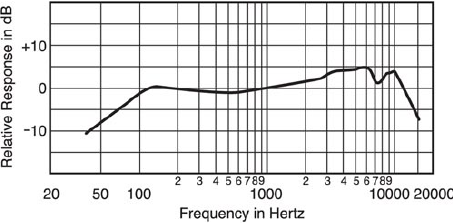
\includegraphics[width=.50\linewidth]{Figures/4 Protocol Design/Frequency Response Range/typical-smartphone-response-range.png}
\end{figure}

Thus, a sound-based move tracking protocol must account for the
following restrictions on which tones can be used for the protocol:

\begin{itemize}

    \item Tones used in the protocol must fall on the range of
    20Hz-20kHz in order to be detectable by a typical smartphone or
    laptop microphone.

\end{itemize}

\subsection{Human Auditory Range}
\label{subsec:human-auditory-range}

An audible protocol could be distracting to a speedcuber. The human ear
can detect audible frequencies from 20Hz to 20kHz, though this usually
degrades with age with many people unable to notice sounds above 16kHz.
\cite{audible-range}. However, not all tones are pleasant to listen to,
particularly higher frequency tones. Tones within the frequency range
of a piano (27.5Hz - 4kHz) are generally considered acceptable, while
tones above the piano's upper range are often irritating.
\cite{piano-range}

Thus, a sound-based move tracking protocol should be considerate of the
human ear's sensitivity to various frequencies:

\begin{itemize}

    \item The most acceptable tones for human speedsolvers are in the
    musical range of up to 4kHz or above the standard audible range of
    16kHz

\end{itemize}


\section{Specification}
\label{sec:specification}

Given the above constraints, this section will detail a sound-based
protocol for tracking the moves of a Rubik's Cube by continuously
transmitting the current state of the cube. In this protocol, changes
to the cube's state cause a change in the transmitted tones which can
be recorded and analyzed to determine the face turn applied.

\subsection{Representing the Cube's Current State}
\label{subsec:representing-cube-state}

As mentioned in Section \ref{sec:rubiks-anatomy}, a Rubik's Cube has
six centerpieces that are fixed relative to each other, but can each
rotate freely through four possible rotational positions as shown in
Figure \ref{fig:rotation-alignment}.

\begin{figure}[h]
    \centering
    \caption{The four possible rotations of a face of a Rubik's Cube \cite{rubiks-turns-images}}
    \label{fig:rotation-alignment}
    \begin{subfigure}{0.25\textwidth}
        \centering
        \caption{Full Alignment}
        \label{fig:rotation-aligned}
        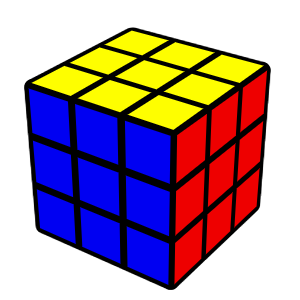
\includegraphics[width=.90\linewidth]{Figures/4 Protocol Design/Specification/fully-aligned.png}
    \end{subfigure}%
    \begin{subfigure}{0.25\textwidth}
        \centering
        \caption{90$^\circ$ Misalignment}
        \label{fig:rotation-misaligned-90}
        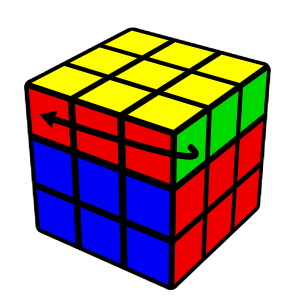
\includegraphics[width=.90\linewidth]{Figures/4 Protocol Design/Specification/90_misaligned.png}
    \end{subfigure}%
    \begin{subfigure}{0.25\textwidth}
        \centering
        \caption{180$^\circ$ Misalignment}
        \label{fig:rotation-misaligned-180}
        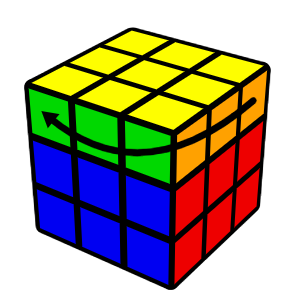
\includegraphics[width=.90\linewidth]{Figures/4 Protocol Design/Specification/180_misaligned.png}
    \end{subfigure}%
    \begin{subfigure}{0.25\textwidth}
        \centering
        \caption{270$^\circ$ Misalignment}
        \label{fig:rotation-misaligned-270}
        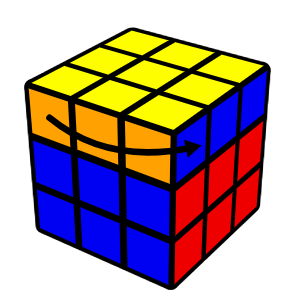
\includegraphics[width=.90\linewidth]{Figures/4 Protocol Design/Specification/270_misaligned.png}
    \end{subfigure}%
\end{figure}

The state of a centerpiece is defined as its current rotational
position. Implicit in this definition is the fact that a centerpiece is
guaranteed to occupy one and only one of its four possible states at
any given time.

Each of the six centerpieces has an independent set of four possible
states, yielding a total of 24 different centerpiece states for the
Rubik's Cube, of which there will always be exactly six active at any
given time.

It's important to note that a knowledge of the current state of each
centerpiece does not imply knowledge of the exact state of each of edge
and corner cubie. For example, after applying the algorithm R U R' U'
all centerpieces have the same state they occupied prior to the
algorithm's execution, while most of the edges and corners in the R and
U layers will have been moved or rotated. However, in the reverse case,
knowledge of the applied move sequence is sufficient information to
determine the exact state of all cubies. Section
\ref{subsec:tracking-face-turns} will explain how extract full move
sequences using only the state information of the centers.

\subsection{Tracking Face Turns}
\label{subsec:tracking-face-turns}

The only way to change a centerpiece's state is by applying a face
turn. As such, when a centerpiece is rotated to a new position, its
state changes to that of the new position. From there, a simple
comparison of the new state to the previous state reveals the exact
face turn applied to the cube.

Thus, in order to determine the sequences of moves applied to the
Rubik's Cube, one simply needs to track how the state of its
centerpieces changes over time.

\subsection{Conveying State Through Sound}
\label{subsec:conveying-state-through-sound}

Conveying the current state of the cube's centerpieces through sound
can be done by simply associating each of the 24 possible centerpiece
states with a specific tone as shown in Table
\ref{table:centerpiece-frequencies} and broadcasting a signal composed
of the six tones corresponding to the active states of the cube's
centerpieces.

Whenever a face turn is applied, the tone associated with the rotated
centerpiece would change to the tone representing the piece's new
state. From there, a microphone equipped device can record the
broadcast frequencies, measure the changes in the frequencies over
time, convert the frequency changes to state changes, and finally
extract any move sequence applied to the cube.

Since there will only ever be a single tone broadcast for a specific
face, the four tones used to represent each of its possible states can
be chosen closer to the minimum separation specified in Section
\ref{subsec:tone-distinctiveness}. However, the gap between tones for
different faces should be larger to help prevent incorrectly
classifying a tone as conveying a state of a different face. In the
sample frequencies shown in Table \ref{table:centerpiece-frequencies},
the frequency gap between faces is 200Hz, a value which performed well
in testing.

\begin{table}[h]
    \centering
    \caption{Sample frequencies for encoding a Rubik's Cube's state}
    \label{table:centerpiece-frequencies}
    \begin{tabular}{ | c | c | c | c | c | c | c | }
        \hline
        Alignment & White & Yellow & Red & Orange & Green & Blue\\
        \hline
        \hline
        Full & 800 Hz & 1300 Hz & 1800 Hz & 2300 Hz & 2800 Hz & 3300 Hz\\
        90$^\circ$ & 900 Hz & 1400 Hz & 1900 Hz & 2400 Hz & 2900 Hz & 3400 Hz\\
        180$^\circ$ & 1000 Hz & 1500 Hz & 2000 Hz & 2500 Hz & 3000 Hz & 3500 Hz\\
        270$^\circ$ & 1100 Hz & 1600 Hz & 2100 Hz & 2600 Hz & 3100 Hz & 3600 Hz\\
        \hline
    \end{tabular}
\end{table}


\section{Alternative Protocol}
\label{sec:alternatives}
% \subsection{Relative Sound Positioning}
% \label{subsec:relative-sound-positioning}

Instead of transmitting the current state of the cube's centerpieces,
an alternative protocol design could seek to directly transmit the face
turns applied to the cube.

This perspective focuses on the fact that all move sequences can be
broken down into a series of 90$^\circ$ face turns. Since the cube
consists of 6 faces, and each face can be turned either clockwise or
counterclockwise, one could design a two-tone protocol using only 8
discrete audio frequencies to build the smart cube. The first tone
would come from one of six predefined audio bands, one for each face of
the cube. The second tone would come from one of two separately
predefined audio bands, one for each possible direction of rotation.
From this, an audio processing model could be designed to process a
sequence of these two-tone pairs and reconstruct the sequence of face
rotations by recording the rotated face followed by its direction of
rotation.

However, while this model minimizes the number of discrete frequencies
required to communicate changes in the cube's state, it carries many
challenges. Consider the example of a speedcuber averaging 5-8 turns
per second (TPS) with bursts up to 20 TPS (common for a speedcuber that
averages under 15 seconds per solution). The burst TPS would require
the successful transmission of 40 sequential tones within a single
second - only 25ms per tone, all in the midst of additional noise from
the cube's pieces hitting each other harder at the higher turn speed.
Adding to the difficulty, since each tone is only ever transmitted
once, the audio detection model must achieve 100\% tone recognition to
be able to accurately reconstruct the originating move sequence. As a
result, this model fails to support any sort of error correction that
would make it resistant to the common challenges to data transmission
through sound.

\newpage
\section{Summary}
\label{sec:protocol-summary}

In summary, a sound based protocol for tracking the moves of a Rubik's
Cube must be considerate of the following constraints:

\begin{enumerate}

    \item Tones should be transmitted with a strength greater than
    -30dB to achieve a high signal-to-noise ratio. (Section
    \ref{subsec:signal-to-noise-ratio})
    
    \item Tones should be separated by at least 100Hz in order to be
    clearly distinguished from other tones in the protocol. (Section
    \ref{subsec:tone-distinctiveness})
    
    \item Tones must fall on the range of 20Hz-20kHz in order to be
    detectable by a typical smartphone or laptop microphone. (Section
    \ref{subsec:frequency-response-range})
    
    \item Tones should fall on the range 0Hz-4kHz or 16kHz-20kHz to
    minimize annoyance to the human speedsolver. (Section
    \ref{subsec:human-auditory-range}).

\end{enumerate}

The protocol that will be used in subsequent chapters consists of 24
unique tones, one for each possible rotational state of each
centerpiece. A transmitter embedded in the Rubik's Cube will
continuously broadcast the six tones corresponding to the current
rotational state of each centerpiece adjust those tones as face turns
are applied (Details in Chapter \ref{Chapter6}). A software receiver
will then listen to the transmitted audio and measure the changes in
the transmitted frequencies over time to reconstruct the originally
applied sequence of face turns (Details in Chapter \ref{Chapter5}).
